%% 
%% Copyright 2016 Icm Ltd
\documentclass[final,3p]{CSP}
\usepackage{enumitem}
\setlist[enumerate]{leftmargin=\parindent,labelindent=\parindent}
\usepackage{amssymb}
\usepackage{changepage}
\usepackage{amsmath}
\usepackage{subcaption}
\usepackage[linesnumbered,vlined,ruled]{algorithm2e}
\SetKwProg{Fn}{Function}{}{}
\begin{document}

\begin{frontmatter}

\title{Systematic Test Case Generation for Augmented Reality Applications}

\author[mymainaddress,mysecondaryaddress]{Richard LaFranchi $<$rlafranc@rams.colostate.edu$>$}

% \author[mysecondaryaddress]{Global Customer Service\corref{mycorrespondingauthor}}
% \cortext[mycorrespondingauthor]{Corresponding author}
% \ead{support@Icm.com}

\address[mymainaddress]{MCS Student, Department of Computer Science}
\address[mysecondaryaddress]{Colorado State University, Fort Collins, Colorado}
\begin{abstract}\rm
\begin{adjustwidth}{2cm}{2cm}{\itshape\textbf{Keyword:}}
Test Generation, Augmented Reality, GUI Ripping, Event Flow Graph, AI Search and Planning
\end{adjustwidth}
\end{abstract}

\begin{keyword}\rm
\begin{adjustwidth}{2cm}{2cm}{\itshape\textbf{Abstract:}}
Augmented Reality (AR) is a type of software that superimposes virtual objects into the physical world.  The reliance that AR has on the physical world makes AR applications difficult to test and very little research exists in the area of testing AR applications.  The objective of this paper is to evaluate if traditional techniques used for test generation on 2D graphical user interfaces (GUI) can be applied effectively to AR applications.  We have developed a systematic method that expands on known techniques in test generation and test automation on traditional 2D GUIs and applies them to 3D objects in an AR environment.  The focus of our research is on test generation but we also demonstrate a method that applies both automated and manual steps to create an end to end test solution for AR applications that can be generalized for most AR applications.  The method is demonstrated on a case study of an AR application that has been developed that detects and measures walls of physical structures such as condo buildings, and commercial buildings.  Given multiple scenarios presented for different structures, we were able to generate a total of \textbf{42,840} feasible test cases and through manual execution of 30 test cases, discovered a total of \textbf{22} faults.  Based on our results we have found that using existing GUI techniques for test generation applied to our method can be effective.  Although our method has been found to be effective, further research and more case studies are recommended for validating our method and to develop more robust methods that can automate the testing process for AR applications.
\end{adjustwidth}
\end{keyword}
\end{frontmatter}

\section{Introduction}
\noindent

Software testing is a broad area of research and it is important to explore existing techniques used in testing software when new types of software emerge.  AR software is one of these areas where testing has not been researched in depth.  Since software is just code, we know that we can apply unit testing appropriately based on existing techniques, but trying to test AR applications from an end to end solution is not as straight forward.  This same problem occurred decades ago in testing GUI applications.  Much of our research here expands on work that A. Memon et al. have done in the area of GUI test automation such as DART \cite{DARTFramework} - Daily Automated Regression Tester, GUI Ripping \cite{GUIRip}, and event-flow graphs \cite{EventFlow}.  Thanks to this existing research we can develop an approach for testing AR applications including a way to automate the generation of test cases.  We will go into further detail about our approach along with the definitions of these concepts.

The purpose of our research is to determine if our approach that applies existing concepts applied to GUI applications can be effective in testing AR applications.  We present the following research question and hypothesis.

\begin{description}
\item[Research Question] Can existing techniques for generating tests in 2D GUI applications be effective in AR applications?
\item[Hypothesis] Using existing techniques for test generation in 2D GUI applications can be applied effectively to AR applications.
\end{description}

In order to confirm our hypothesis, we will use our approach and present a case study on a developed AR application that has been built using XCode \cite{xcode} and Apple's ARKit \cite{ARKit} for developing mobile AR applications that can be run on iPhones and iPads.  The programming language used for the application is Swift \cite{swift} and the algorithms presented in our approach are implemented as Swift code directly in the application code.  Although our approach is applied using Swift code, the algorithms can be generalized to be able to apply to any programming language or environment.  The application developed is a tool for detecting and measuring vertical walls in physical structures.  The approach relies on presenting a scenario as an initial state that includes a physical structure and that at least one virtual wall has been overlaid in the physical environment.  We will run our method on multiple scenarios and report the generated test cases.  We will attempt to manually execute the test cases generated in hopes to discover faults present in the application.

The audience intended for this research is other researchers or professionals who are working on projects in AR or also Virtual Reality (VR).  We believe that the concepts and method presented will also be applicable to VR software.  Our approach presented should also be a practical way for those looking to incorporate a more formal testing process in developing AR and VR software.

\section{Approach}
\noindent
Our approach involves a systematic combination of manual and automated steps for generating test cases in AR applications.  For those who do not come from a testing background is important to understand how to do test design and some of the definitions needed to understand software testing.  We will cover definitions in software testing as well as definitions that apply specifically to research in GUI testing and how we can expand on the definitions to come up with an approach for test generation.

At a high level, our method involves setting an application up in an initial state where 3D objects are visible, running a depth-first traversal algorithm (aka GUI Ripper \cite{GUIRip}) to extract the structure of the virtual nodes in the application, building an event-flow graph \cite{EventFlow} based on the structure extracted, and then based on a goal state, find one or more paths in the event-flow graph that make up our test cases.  We will go into more detail on these steps and the algorithms involved for test generation in this section.  Although our method does not specifically rely on AI search and planning, we will discuss this topic and potential applications of AI in the test generation method.

Our method will be applied to a case study of an AR application developed that measures the exterior of physical structures along with the results that we found.  The metrics we are evaluating as dependent variables in this case study will be the number of test cases generated and number of faults detected through manual testing.  The independent variables of the case study will be type of physical structure and the number of virtual walls presented as an initial state.  More details about the scenarios used and the results obtained in the case study will be presented in this section.

\subsection{Definitions}
\noindent

Definitions are provided verbatim from appropriate citations unless otherwise noted.  We are documenting important terms so that our method is easier to understand for those who are interested in our method but don't have a background in software testing.  Below we also provide definitions more specifically related to research on testing GUI applications.  We provide a thorough evaluation on these definitions and how they can be applied to an AR environment.

\begin{description}
\item[Software Fault] \cite{intrototesting} defines as "A static defect in the software".
\item[Software Error] \cite{intrototesting} defines as "An incorrect internal state that is the manifestation of some fault".
\item[Software Failure] \cite{intrototesting} defines as "External, incorrect behavior with respect to the requirements or other description of the expected behavior".
\item[Expected Results] \cite{intrototesting} defines expected results as "The result that will be produced when executing the test if and only if the program satisfies its intended behavior".
\item[Prefix Values] \cite{intrototesting} defines prefix values as "Any inputs necessary to put the software into
the appropriate state to receive the test case values". 
\item[Postfix Values] \cite{intrototesting} defines postfix values as "Any inputs that need to be sent to the software after the test case values are sent".
\item[Test Case] \cite{intrototesting} defines a test case as "composed of the test case values,
expected results, prefix values, and postfix values necessary for a complete execution and evaluation of the software under test".
\item[Generator] \cite{intrototesting} defines a generator as a "procedure that automatically generates values to satisfy a criterion".  Since this term is very broad, we are more specifically interested about test generation which in my own terms is the process of generating one or more test cases where the definition of a test case is fulfilled be the provided definition.
\item[GUI Ripping] Based on \cite{GUIRip} we can summarize the definition of GUI ripping as the process of extracting the hierarchical structure of a GUI in terms of windows, widgets, properties of the widgets, and values of said properties.
\item[GUI Forest] Based on \cite{GUIRip} we can summarize a GUI Forest as the hierarchical structure extracted from the GUI ripping process defined as the set of windows, widgets, properties, and values.  We can apply this definition to an AR environment in terms of the hierarchical structure of virtual objects and their properties such as shape, size, orientation, etc. within an AR window which we can define as an AR Forest.
\item[Event-flow Graph] \cite{GUIRip} and \cite{EventFlow} provide slightly different definitions as they apply to GUI components or dialogues, so we can summarize and event-flow graph as a graphical representation of events and relationships between events.  In traditional GUI applications interactions or events that occur with widgets such as buttons typically only have possible event available.  This is not the case where virtual objects in an AR environment could be interacted with in multiple ways.  We provide further examples of event-flow graphs in our method and as it applies to our case study in sections 2.2 and 2.3.
\end{description}

\subsection{Test Generation Method}
\noindent

Our test generation method can be described in the following three sections as a combination of automating the described algorithms along with our process of including manual steps to complete the process.  We will provide more in depth details about the depth-first traversal algorithm, building the event-flow graph, test generation and path finding algorithms, and our step-by-step guide for test generation and test execution.

\subsubsection{Depth-first Traversal Algorithm for GUI Ripping}
\noindent

\cite{GUIRip} presents depth-first search algorithms as shown in Figure \ref{alg:gui-dfs}.  The algorithms use concepts such as windows and widgets which are commonly used in GUI applications.  In an AR applications, these algorithms translate easily over to 2D objects that may exist, but we want to modify the algorithms to support 3D objects that occur in the AR environment.  We present Algorithms \ref{alg:dfs} and \ref{alg:dfs-recursive} which translate these algorithms in terms of 3D virtual objects. The purpose of these algorithms is to discover the hierarchical structure and extract it into an AR Forest. These algorithms do not build the event-flow graph, but rather extract the structure in order to assist in building the event-flow graph. Algorithm \ref{alg:dfs} begins by simply looping through each virtual object currently present in an AR Window and passes the node to the the recursive Algorithm \ref{alg:dfs-recursive}.

\begin{figure}[h]
\caption{GUI Ripping Algorithms from \cite{GUIRip}} 
\centering
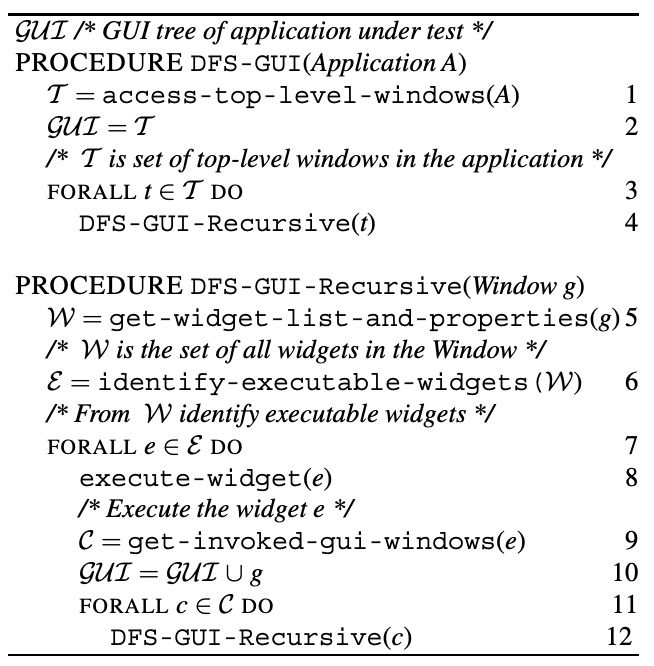
\includegraphics[width=0.7\textwidth]{DFS-GUI.png}
\label{alg:gui-dfs}
\end{figure}

\begin{algorithm}
    \SetKwInOut{Input}{Input}
    \SetKwInOut{Output}{Output}
    \Input{The AR Forest}
    \Output{No output}
    \Fn{DFS-AR (forest)} {
      \tcc{topLevelNodes are the currently present virtual objects in the AR Window}
      \For{node in forest.topLevelNodes}{
        DFS-AR-Recursive(node)
      }
    }
    \caption{Our modified version of the GUI Ripping algorithm}
    \label{alg:dfs}
\end{algorithm}

\begin{algorithm}
    \SetKwInOut{Input}{Input}
    \SetKwInOut{Output}{Output}
    \Input{A Virtual Object or Node in the AR Environment}
    \Output{No output, structure of the forest is updated at each level}
    \Fn{DFS-AR-Recursive (node)} {
      \If{isExecutable(node)}{
        \tcc{Virtual objects may support one or more different types of events}
        \For{eventType in eventTypesFor(node)}{
            \tcc{Execute the event on the node}
            execute(node, eventType)\;
            \tcc{invokedNodes() is a method that finds any new virtual objects in the AR Window that appear}
            children= invokedNodes()\;
             \tcc{Update the structure so that invoked nodes are added as children to the current node}
            node.addChildren(children)\;
            \For{child in children} {
                DFS-AR-Recursive(child)\;
            }
        }
      }
    }
    \caption{Our modified version of the recursive GUI Ripping algorithm}
    \label{alg:dfs-recursive}
\end{algorithm}

The biggest difference between our algorithms and the GUI Algorithms, is that for one we are dealing with 3D virtual objects, and the second is that these objects may support other types of events.  In a 2D GUI application, a widget such as a button may only support one type of event such as a click event.  In an AR environment, many different types of events or triggers could be supported.  The events supported will be domain specific as well as hardware specific.  The AR application may support a gesture set for performing different actions.  If the AR application doesn't have a limit on the potential number of objects that may appear in the environment, it is important to add a maximum depth-level to the algorithm, otherwise it will run into a stack overflow error.

\subsubsection{Building the Event-flow Graph}
\noindent
An event-flow graph is simply a directed graph that holds a set of vertices representing events and edges between events.  A path in the graph represents a sequence of events.  Figure \ref{fig:evt-flow} shows an example of an event-flow graph discovered in the case study which will be discussed further in section 2.3. Once we have knowledge about the structure of the virtual objects extracted during the ripping phase, we can create an event-flow graph based on the virtual objects that allow interaction. \cite{EventFlow} presents the getFollows() algorithm as shown in Figure \ref{alg:gui-getFollows} which determines how to build the edges or events that follows a particular event.  Similar to the GUI Ripping algorithms much of the concepts presented in the algorithm refer to concepts that apply to 2D GUI widgets.  In this algorithm, B refers to what is known as a GUI component.  A component an AR environment could be defined as a group of similar virtual objects.  Out approach doesn't specifically evaluate components and assumes AR windows and components are one in the same.  So the algorithm for our approach simplifies to return all other objects in an AR window.

Often times in an AR environment you have multiple objects available, so the next event that can occur could happen with any of these objects available.  In this case, edges in the event flow graph that follow a particular event are all possible edges to the other objects in the environment.  A simple algorithm can be executed to just add an edge to and from for every possible pairs of vertices or events in the graph.

\begin{figure}[h]
\caption{Get Follows Algorithm from \cite{EventFlow}} 
\centering
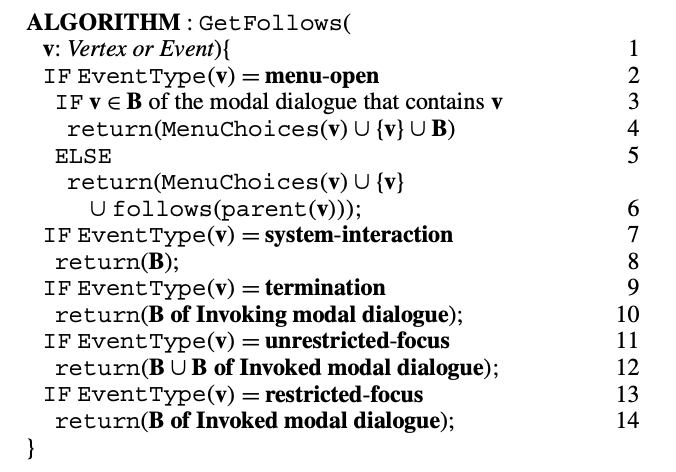
\includegraphics[width=0.7\textwidth]{getfollows.png}
\label{alg:gui-getFollows}
\end{figure}

\subsubsection{Test Generation and Path Finding Algorithms}
\noindent

Once we have constructed our event-flow graph, we can use a path finding algorithm to generate possible sequences of events otherwise known as test cases.  The simplest approach is to simply find all possible paths in the event flow graph given a source and a destination as shown by Algorithm \ref{alg:getAllPaths}.  Algorithm \ref{alg:generatetests}
 presents a way to use the path finding algorithm by using each top level node in the event-flow graph as a potential source and allows us to have a way to export the generated testes.  This is a naive approach since it generates all possible paths in the graph.  It may potentially create infeasible paths for one reason or another.  Although the approach works well for our case study, it may not work well on other AR applications.  So we would like to present other options that use AI Search and Planning approaches to path finding.
 
Memon, A. recommends using planning and AI in \cite{framework} for finding test case paths.  At a high level, given an initial state in the software, provide a goal state and AI will learn how to reach the goal state.  In the context of GUI applications, this appears to be more feasible since the state space is relatively small.  In AR, the state space is infinitely large, since you could have virtual objects that could potentially support multiple types of transformations.  In a finite state space, you could run a simple breadth-first search to find a goal state, or even just select next events to perform randomly over many iterations to find possible paths to reach a goal state.

In generating test cases as shown in Algorithm \ref{alg:getAllPaths}, we could modify this slightly, to instead accept goal conditions for our event-flow graph to find a valid path, instead of only providing a destination event.  For our case study, finding all paths that visit every node once was sufficient since the application only supports selection events and the state space is relatively small, but does create paths that are infeasible as we will show in section 2.4.  Planning in AI is slightly different from searching, in searching you are searching through the state space of an application, where in planning, you search through a plan space to incrementally create a plan that achieves a goal state.

 
\begin{algorithm}
    \SetKwInOut{Input}{Input}
    \SetKwInOut{Output}{Output}
    \Input{The event-flow graph, a source event, a destination event, a path list holding the sequence of events, a paths list holding a list of paths}
    \Output{No output, the paths list holds the list of tests generated}
    \Fn{getAllPaths (graph, source, destination, path, paths)} {
      source.visited = true\;
      path.append(source)\;
      \eIf{$source=destination$}
      {
        paths.append(path)\;
      }
      {
        \For{neighbor in graph.neighbors(source)}{
            \If{$neighbor.visited = false$}{
                getAllPaths$(graph, neighbor, destination, path, paths)$\;
            }
        }
      }
      path.pop()\;
      source.visited = false\;
    }
    \caption{Simple path finding Algorithm that finds all paths between a source event and a destination event in an event-flow graph}
    \label{alg:getAllPaths}
\end{algorithm}

\begin{algorithm}
    \SetKwInOut{Input}{Input}
    \SetKwInOut{Output}{Output}
    \Input{The event-flow graph}
    \Output{No output, paths list can be used to export data to a desired format}
    \Fn{generateTestCases (graph)} {
        \tcc{Last event in the graph is the destination}
        destination = graph.vertices[graph.vertices.length-1]\;
        paths = []\;
        \For{node in graph.topLevelNodes}{
            path = []\;
            getAllPaths$(graph, node, destination, path, paths)$\;
        }
        \tcc{export paths to desired format}
        exportData(paths)\;
    }
    \caption{Algorithm that loops through the top-level virtual objects and uses getAllPaths to generate the tests}
    \label{alg:generatetests}
\end{algorithm}

\subsubsection{Combining Manual and Automated Steps}
\noindent

For any given AR application we can perform the following steps to generate test cases for an individual scenario.  This process relies on some domain knowledge and assumes some test design has been performed for a particular scenario such that prefix values, postfix values, and expected results are already determined for a particular scenario.

\begin{enumerate}
    \item Manually bring the AR environment so that Prefix values are met
    \item Execute the test generation by running and automating the following algorithms in order
    \begin{enumerate}
        \item Rip the GUI by running Depth-first traversal algorithm
        \item Based on the structure extracted, run an algorithm to build the event-flow graph
        \item run path finding algorithm on the event-flow graph
        \item report paths generated as test cases to be used in manual execution.
    \end{enumerate}

\end{enumerate}

Once tests have been generated, manual execution of the test cases is achievable.  It is important to note that we must define possible failures in the application ahead of time which will help us evaluate expected results.  Before we begin execution it is also important to manually inspect the tests to determine feasibility and be able to filter out infeasible paths generated.  To execute the tests manually perform the following steps:

\begin{enumerate}
    \item For each feasible generated test case:
    \begin{enumerate}
        \item setup prefix conditions
        \item For each event in the test case:
        \begin{enumerate}
            \item execute event
        \end{enumerate}
        \item Check expected results and record failures if the test produced faulty results
        \item setup postfix conditions or return application to a clean state
    \end{enumerate}
\end{enumerate}

In the next section we go into more details about our case study and how we used it to apply our method and evaluate our approach.

\subsection{Case Study}
\noindent

To implement our test generation method, we developed an iOS application using XCode written in the Swift programming language and the ARKit tool-set for developing iOS AR applications and tested the implementation on an iPhone 7.  The application is designed to be a measurement tool for civil engineers, land surveyors, or building architects who need to measure the exterior of a physical structure for building planning or other purposes.  The application uses vertical plane detection techniques to find walls on a structure, displays those walls as virtual objects, which can be selected.  Once walls are selected, the intersection of the planes are calculated and virtual spherical objects appear at the intersection denoting building corners.  Corners can then be selected and lines between the corners along with some text showing the dimensions of the building in feet will appear based on the corners that are selected.  Figure \ref{fig:blda} shows how the virtual walls appear in the environment and \ref{fig:meas} shows how the building lines and measurements between walls appears.  The virtual walls and corners appear green when selected.

In order to determine effectiveness of our test generation method, it is important to determine what constitutes a software fault as it applies to our application.  In our application we can determine three different types of failures that could occur:

\begin{enumerate}
    \item Measurement Inaccuracy +/- 0.5 ft
    \item Representation Inaccuracy
    \item System Failure (Crashes, Freezes, or Other)
\end{enumerate}

A measurement inaccuracy occurs when the representation of our building or structure is correct, that is the building lines that appear represent the shape of the structure correctly, however the actual measurements are inaccurate.  A representation inaccuracy is one in which the representation of the building is incorrect.  A system failure is some other failure that may occur below the application and cause the application to crash.

Our case study sets up prefix conditions by manually walking around a structure until the appropriate number of walls appear.  A button in the application is implemented in order to trigger the ripping and generation process.  It exports the data as a CSV file similar to the data shown in table \ref{tab:3walls}.   These tests are then executed and any failures that are discovered are recorded for the test case.  It uses the number of walls as a prefix value for our main independent variable and the actual structure as another independent variable.  The dependent variables are the number of tests generated and the number of faults detected during manual execution of the tests.  We will also not the number of paths that are infeasible.

\begin{figure*}[t!]
    \centering
    \begin{subfigure}[t]{0.6\textwidth}
        \centering
        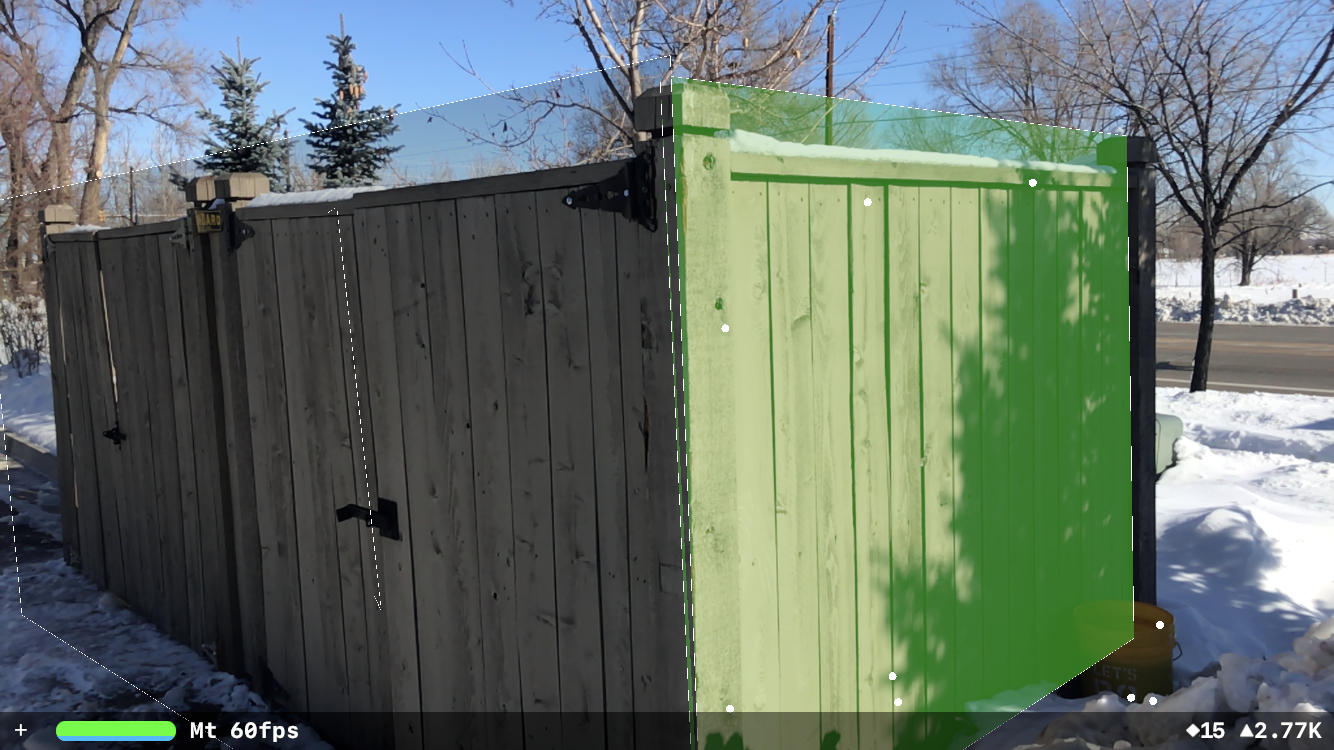
\includegraphics[height=2.0in]{building-a.PNG}
        \caption{Building A - Wood Frame Trash Enclosure}
        \label{fig:blda}
    \end{subfigure}%
    ~ 
    \begin{subfigure}[t]{0.4\textwidth}
        \centering
        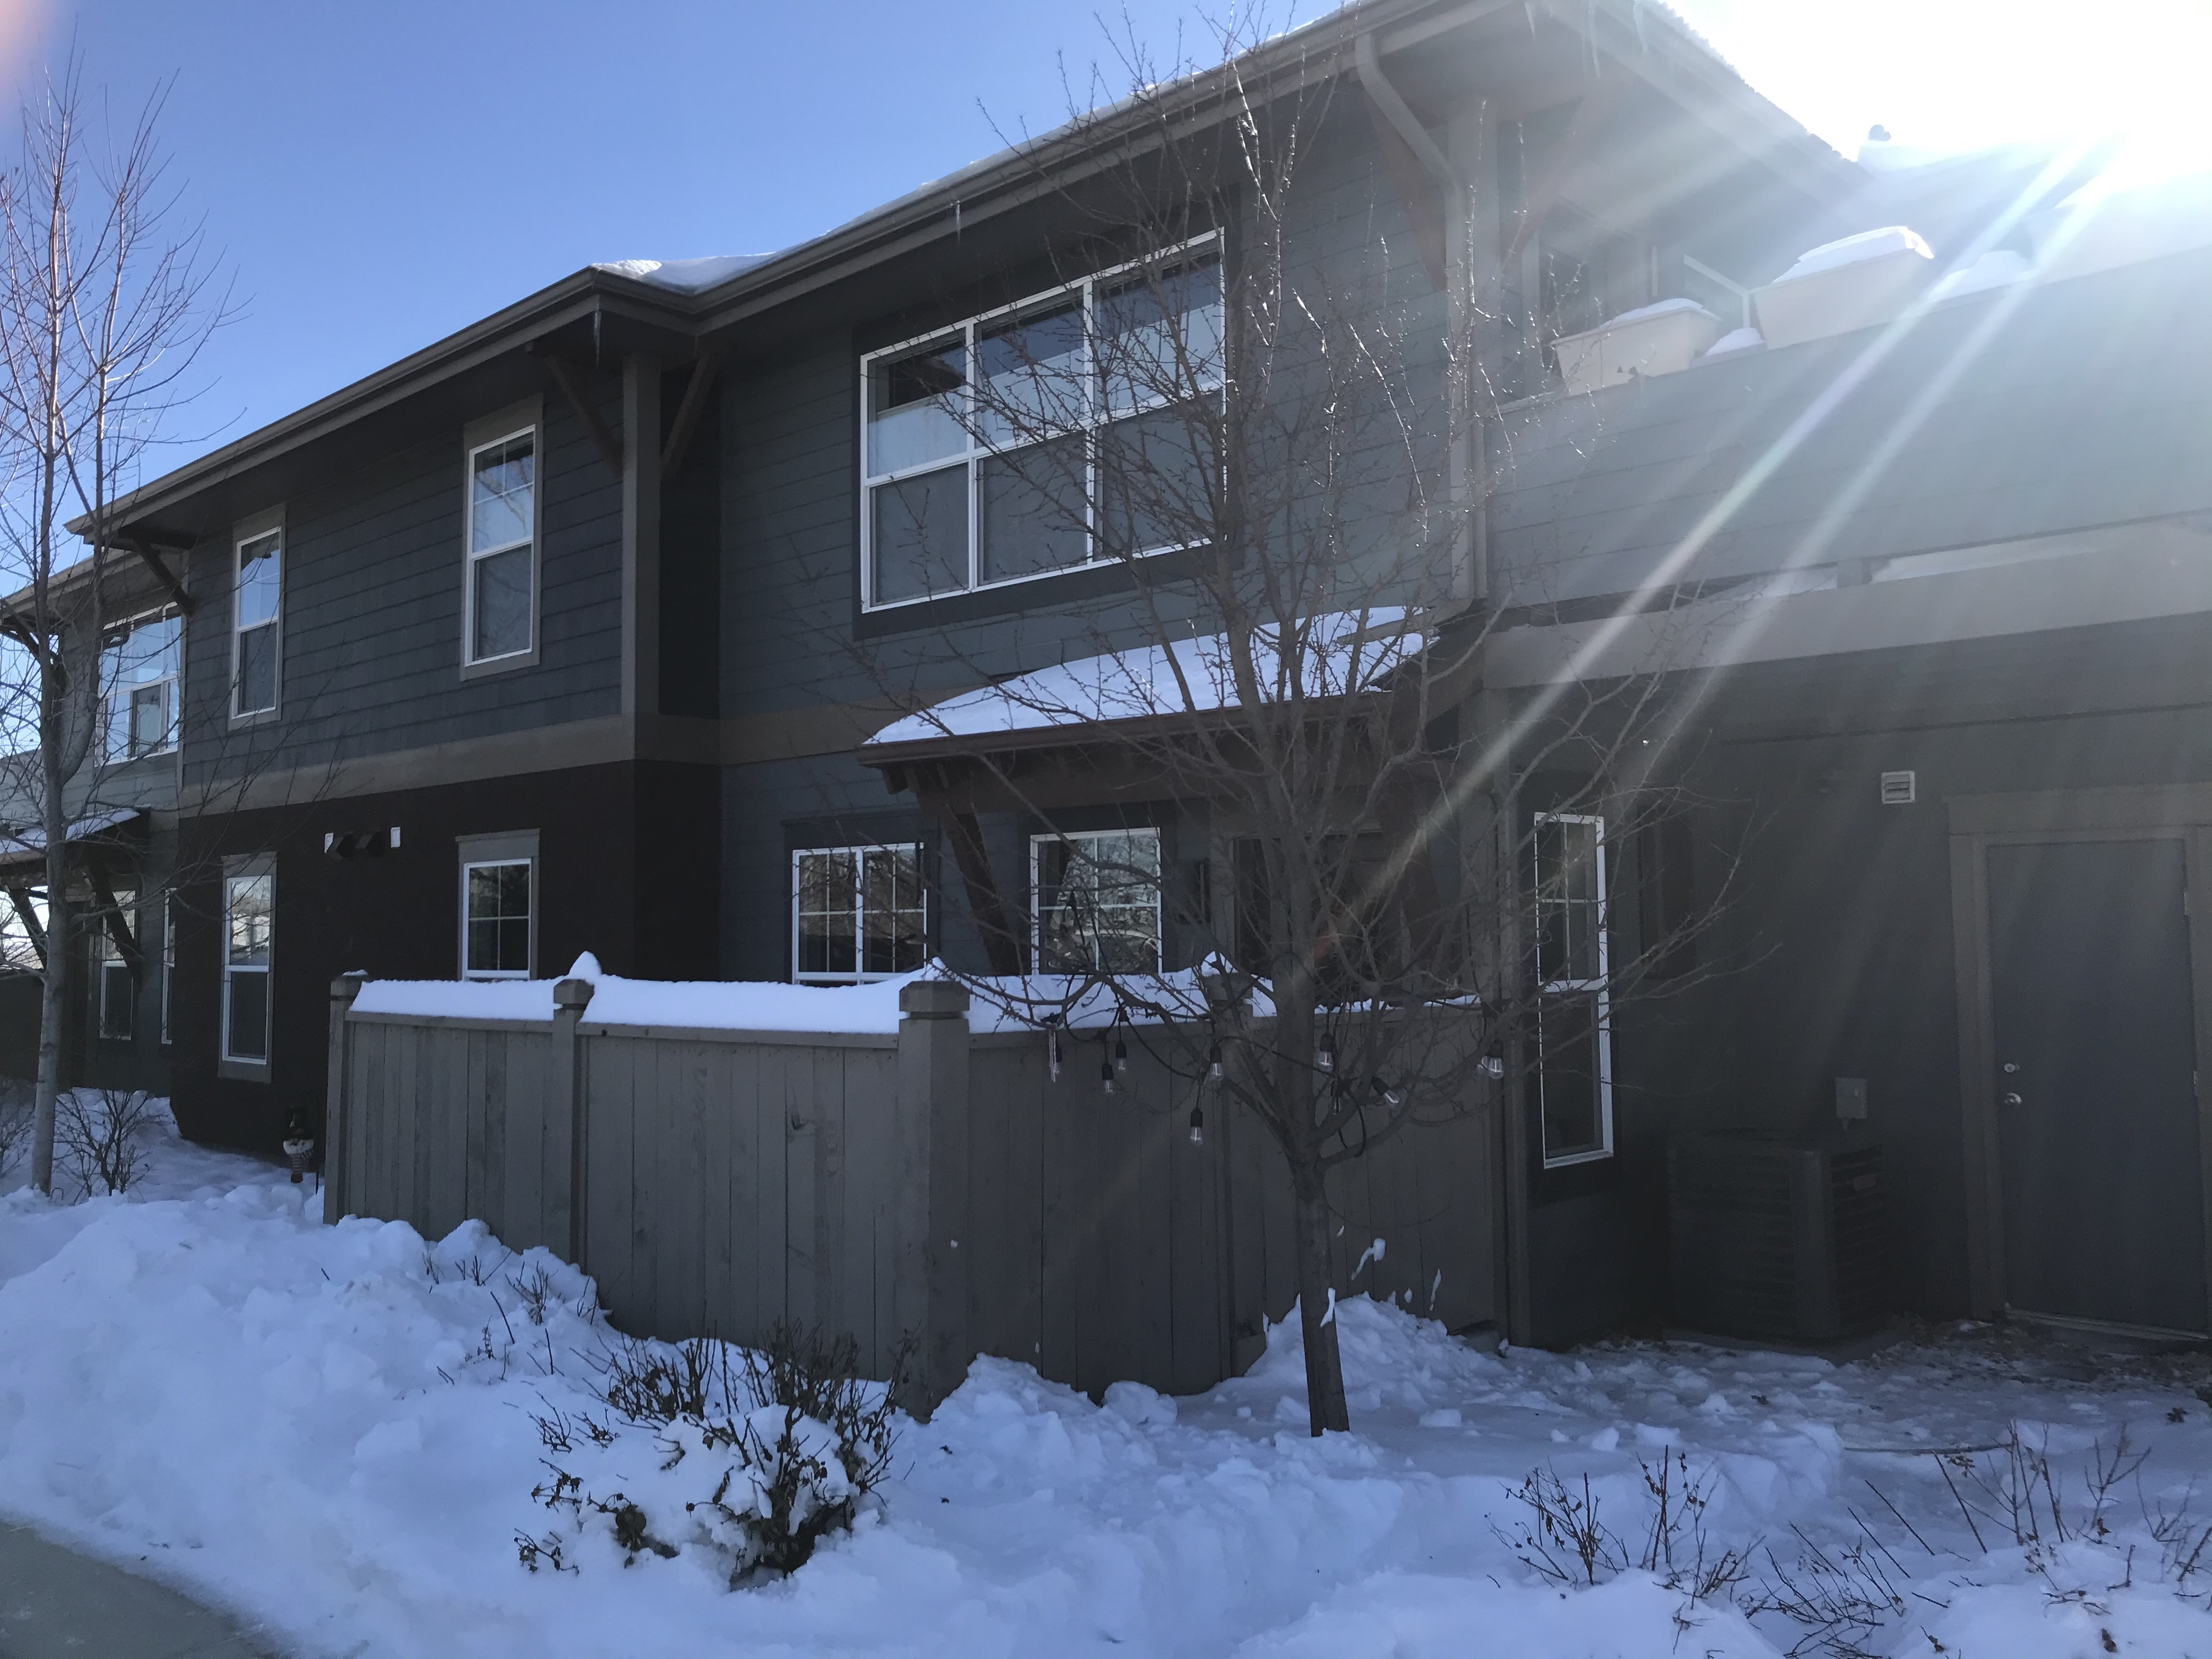
\includegraphics[height=2.0in]{building-b.jpg}
        \caption{Building B - Two Story 8 Unit Wooden Frame Condo Building}
        \label{fig:bldb}
    \end{subfigure}
    \caption{Buildings Tested for Case Study}
\end{figure*}

\begin{figure*}[t!]
    \centering
    \begin{subfigure}[t]{0.5\textwidth}
        \centering
        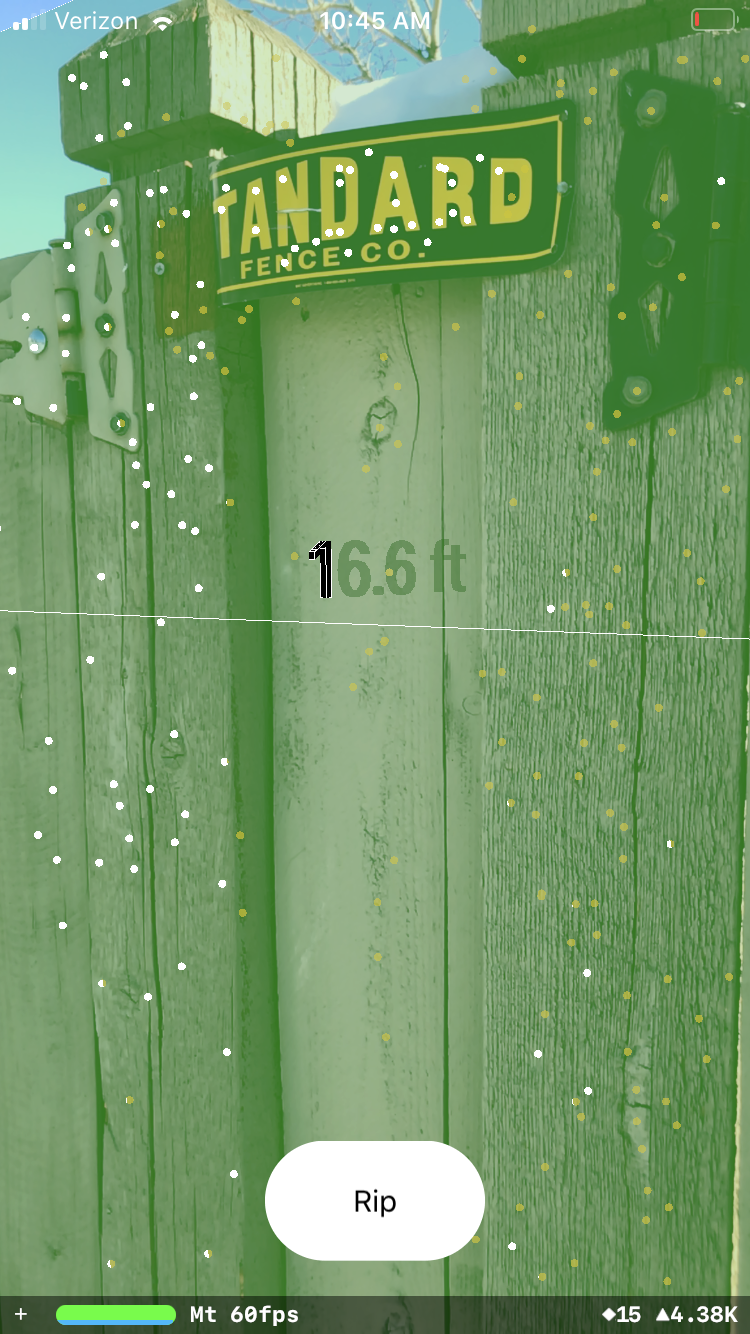
\includegraphics[height=5.0in]{measurement-example.PNG}
        \caption{Measurement Display of Wall 2 on Building A}
        \label{fig:bldam}
    \end{subfigure}%
    ~ 
    \begin{subfigure}[t]{0.5\textwidth}
        \centering
        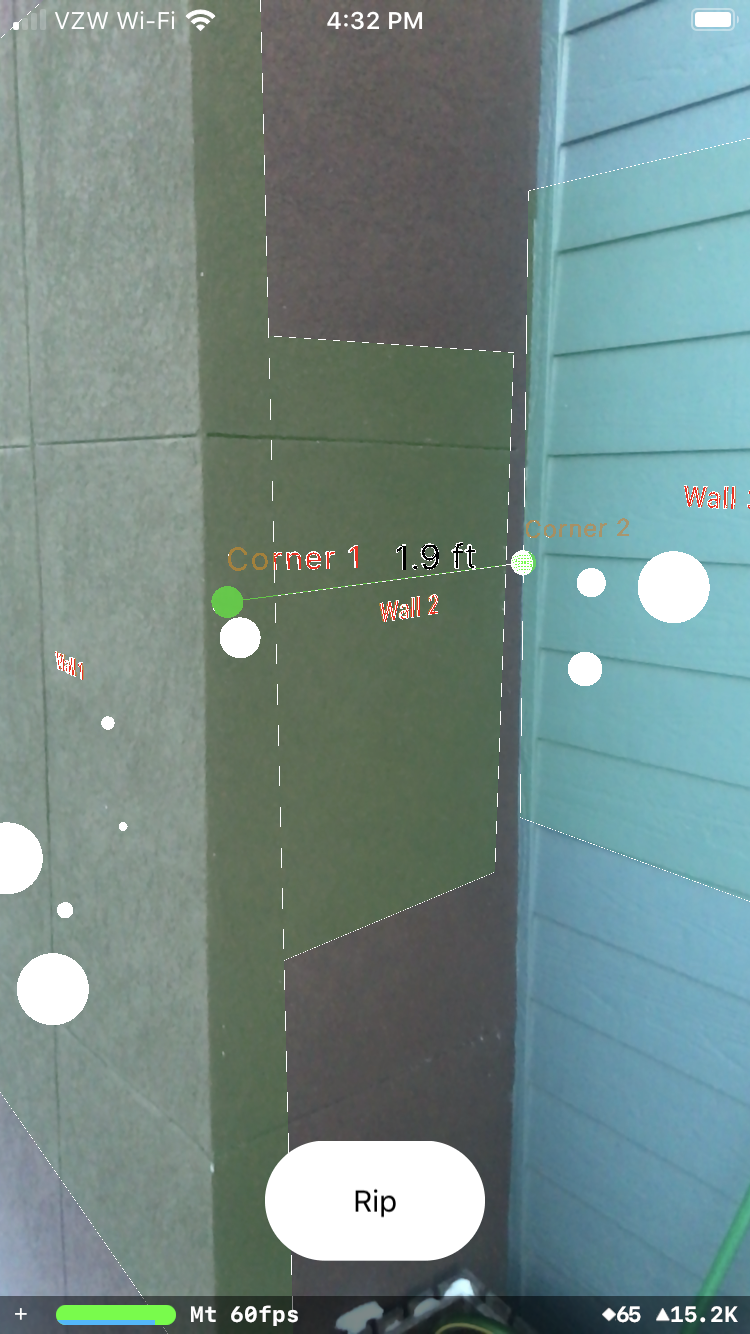
\includegraphics[height=5.0in]{meas-bldb.PNG}
        \caption{Display after Ripping Process Executes on Building B}
        \label{fig:bldbm}
    \end{subfigure}
    \caption{Application Examples}
\end{figure*}

We performed our experiment on 4 different scenarios on two different structures as shown in Figure \ref{fig:blda} and \ref{fig:bldb} referred to as Building A and Building B respectively.  Building A is a rectangular wooden trash enclosure so it only has 4 walls.  Building B is a two story wooden frame condo building with 8 condo units.  Building B has a total of 36 walls, but we ran our method on a partial section of the building on a scenario of 5 walls for prefix conditions. A building detail of the 5 walls of Building B are shown in Figure \ref{fig:bldBdetail}.  On Building A, our method was executed on scenarios of 2,3, and 4 walls for prefix conditions.  The conditions during the experiment were snow covered ground, sunny with an approximate temperature of 30 degrees Fahrenheit.

All of the feasible tests for 2 and 3 walls prefix values were executed.  A subset of 10 feasible tests for each the prefix values of 4 walls and 5 walls were chosen at random for execution.

To determine measurement inaccuracies, the building walls that we tested on were physically measured with a tape measure to the nearest tenth of a foot.  The summary of these measurements are shown in Table \ref{tab:meas}.  A measurement failure was recorded if a representation failure did not occur and the measurement seen of a wall as shown in Figure \ref{fig:bldam} and Figure \ref{fig:bldbm} had a larger error of 0.5 feet.  When the ripping process is completed it is necessary to label the virtual objects as shown in \ref{fig:bldbm} so that we know which events corresponds to which virtual objects so that tests can be executed on the appropriate objects.

\begin{table}[]
    \centering
    \begin{tabular}{c|c|c}
         Wall & Building A & Building B  \\
         Wall 1 & 7.9' & N/A \\
         Wall 2 & 17.0' & 10.1' \\
         Wall 3 & 8.0 & 4.0' \\
         Wall 4 & 16.9 & 12.8' \\ 
    \end{tabular}
    \caption{Wall Measurements}
    \label{tab:meas}
\end{table}

Since the application developed is a prototype it is expected to be very faulty so we expect to find a high percentages of faults in our results by using our method.  We will evaluate results in the next section.

\subsection{Results}
\noindent

Table \ref{tab:results} summarizes the results for each scenario and as shows that we generated a total of 1,817,300 test cases, 42,840 of which are feasible.  Due to time constraints for manual execution only 30 of tests were executed.  Out of the 30 tests, 22 of the tests produced faults.  16 of these faults were from representation failures and 5 of these faults were from failures in measurement inaccuracies.  1 test was recorded as a system failure because of an inability to select a corner during the process.  This prevented further execution of the test case. 8 of the tests passed with measurement and representation confirmations.   All of the 4 walls and 5 walls tests failed mostly due to representation errors.  In the 4 walls scenario this occurred when a measurement line appeared diagonally across the structure for example when corners 1 and 3 were selected in order.  Our tests during the prefix values of 5 walls lead to the discovery that additional corners appeared where true building corners did not exist leading to representation failures.  The high percentage of faults produced confirmed our expectation because the application is in a prototype phase.

A closer evaluation of the scenario with a 3 walls prefix on Building A reveals more details about the tests generated as shown in Table \ref{tab:3walls}.  All of the tests conclude with selecting corner 2 as the last event, which makes sense because this is the last vertex that is added to the event-flow graph.  Also, any events where event 2 contains a selection of corner 1 is not feasible since at least 2 walls must be selected in order for a corner to appear.  This leaves feasible paths to be any path where selecting corner 1 is the third event and the first 2 events contain walls 1 and 2.   This is true because walls 1 and 2 must be selected in order for corner 1 to appear.  This leaves test cases 1, 2, 5, 7, 8, 11, 13, and 15 in Table \ref{tab:3walls} for a total of 8 feasible paths out of 18 generated.  The event-flow graph created by running our algorithms as shown in Figure \ref{fig:evt-flow} shows that our events contain edges in both directions to every other event in the graph.  However, depending on the state of the application, certain edges may or may not be available at a particular point in time.  Showing that only a portion of the tests generated for the 3 walls prefix condition is a good example of this.

As we increase the number of walls for a scenario we can see that the percentage of feasible tests drops.  For example, with 4 walls, approx. 10\% out of 2880 tests generated are feasible and looking at 5 walls, approx. 2\% of 1,814,400 tests cases generated were feasible.  Since the prefix value of 3 walls had a small enough number of test cases, feasibility could be determined by manual inspection.  The feasibility of the test cases for 4 and 5 walls were determined programmatically.

We want to determine if the tests generated on the 5 walls prefix scenario were the result of a flaw in our ripping process or were actual faults.  We see that our tests generated include additional corners that shouldn't appear in the scenario as shown in Figure \ref{fig:bldBdetail}.  Here is an example Test Case that was generated:

\begin{description}
  \item[Test 1: 5 Walls Prefix] SELECT Wall 1, SELECT Wall 2, SELECT Wall 4, SELECT Corner 3, SELECT Wall 3, SELECT Corner 1, SELECT Corner 2, SELECT Wall 5, SELECT Corner 5, SELECT Corner 6
\end{description}

This test reveals that two extra corners are included beyond the expected 4 corners based on the physical structure of the building.  By manual inspection we determined that this was in fact the result of a fault in the software and not in the ripping process.  Since the application determines the location of corners based on the intersection of vertical planes, it would calculate the intersection of corners that didn't actual exist physically.  As shown in figure \ref{fig:bldBdetail}, we see that corner 3 appears because it intersects walls 1 and 4. Corner 5 appears at the intersection of walls 2 and 5.  This confirms that the representational failures discovered during testing Building B were in fact the result of actual faults in the software.

\begin{figure}
    \centering
    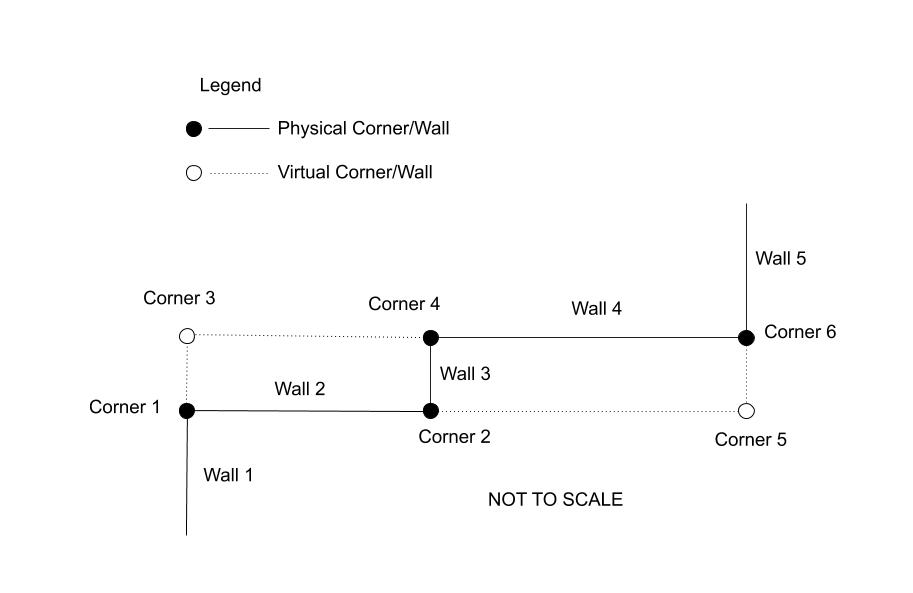
\includegraphics[width=\textwidth]{Building5detail.jpg}
    \caption{Building Detail of 5 Walls Tested on Building B}
    \label{fig:bldBdetail}
\end{figure}

We can confirm the effectiveness of our method by that fact that we were able to generate a large number of feasible test cases, however there exists many threats to validity.  The biggest threat is that our application is faulty because of the prototype phase it is in and of the specific use case that it applies to.  It is hard to determine if our approach can be generalized to other use cases and AR applications.  Also, because of time limitations in manual test execution it is difficult to determine percentage of faults over all of the feasible test cases generated.  We can only evaluate this over the test cases that were actually executed.

\begin{figure}
    \centering
    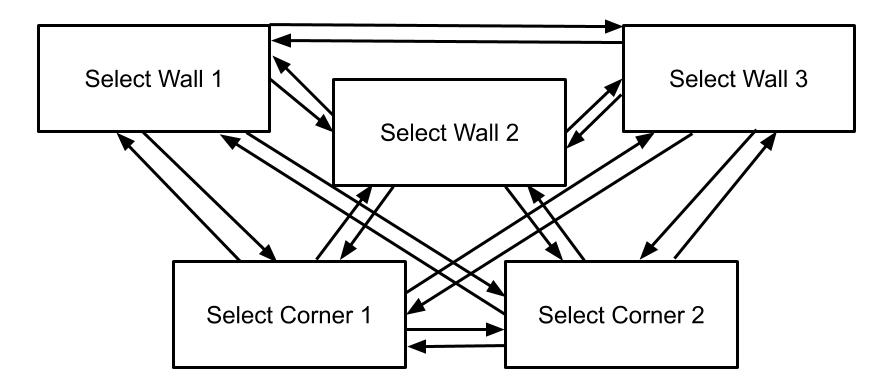
\includegraphics[width=0.7\textwidth]{Event-Flow.jpg}
    \caption{Event-flow Graph from a Prefix Condition of 3 Walls}
    \label{fig:evt-flow}
\end{figure}

\begin{table}[]
    \centering
    \begin{tabular}{ |p{2cm}|p{1cm}|p{1cm}|p{1cm}|p{1cm}|p{2cm}| }
     \hline
      \multicolumn{1}{|c|}{Building} &
      \multicolumn{3}{|c|}{Building A} &
      \multicolumn{1}{|c|}{Building B} &
      \multicolumn{1}{|c|}{} \\
     \hline
      \multicolumn{1}{|c|}{Prefix} &
      \multicolumn{1}{|c|}{2 Walls} &
      \multicolumn{1}{|c|}{3 Walls} &
      \multicolumn{1}{|c|}{4 Walls} &
      \multicolumn{1}{|c|}{5 Walls} &
      \multicolumn{1}{|c|}{\textbf{Total}}
      \\
     \hline
     Tests Gen. & 2 & 18 & 2880 & 1,814,400 & 1,817,300 \\
     \hline
     Feasible & 2 & 8 & 272 & 42,560 & 42,840 \\
     \hline
     Executed & 2 & 8 & 10 & 10 & 30 \\
     \hline
     Faults & 0 & 2 & 10 & 10 & 22 \\
     \hline
     \hline
     Meas. F. & 0 & 2 & 3 & 0 & 5 \\
     \hline
     Repr. F. & 0 & 0 & 6 & 10 & 16 \\
     \hline
     System F. & 0 & 0 & 1 & 0 & 1 \\
     \hline
    \end{tabular}
    \caption{Summary of Tests Generated}
    \label{tab:results}
\end{table}

\begin{table}[]
    \centering
    \begin{tabular}{|p{2cm}|p{2cm}|p{2cm}|p{2cm}|p{2cm}|p{2cm}|}
    \hline
     Test Case No. & Event 1 & Event 2 & Event 3 & Event 4 & Event 5  \\
     \hline
    1 & SELECT Wall 1 & SELECT Wall 2 & SELECT Corner 1 & SELECT Wall 3 & SELECT Corner 2 \\
    \hline
    2 & SELECT Wall 1 & SELECT Wall 2 & SELECT Wall 3 & SELECT Corner 1 & SELECT Corner 2 \\
    \hline
    3 & SELECT Wall 1 & SELECT Corner 1 & SELECT Wall 2 & SELECT Wall 3 & SELECT Corner 2 \\
    \hline
    4 & SELECT Wall 1 & SELECT Corner 1 & SELECT Wall 3 & SELECT Wall 2 & SELECT Corner 2 \\
    \hline
    5 & SELECT Wall 1 & SELECT Wall 3 & SELECT Wall 2 & SELECT Corner 1 & SELECT Corner 2 \\
    \hline
    6 & SELECT Wall 1 & SELECT Wall 3 & SELECT Corner 1 & SELECT Wall 2 & SELECT Corner 2 \\
    \hline
    7 & SELECT Wall 2 & SELECT Wall 1 & SELECT Corner 1 & SELECT Wall 3 & SELECT Corner 2 \\
    \hline
    8 & SELECT Wall 2 & SELECT Wall 1 & SELECT Wall 3 & SELECT Corner 1 & SELECT Corner 2 \\
    \hline
    9 & SELECT Wall 2 & SELECT Corner 1 & SELECT Wall 1 & SELECT Wall 3& SELECT Corner 2 \\
    \hline
    10 & SELECT Wall 2 & SELECT Corner 1 & SELECT Wall 3 & SELECT Wall 1 & SELECT Corner 2 \\
    \hline
    11 & SELECT Wall 2 & SELECT Wall 3 & SELECT Wall 1 & SELECT Corner 1 & SELECT Corner 2 \\
    \hline
    12 & SELECT Wall 2 & SELECT Wall 3 & SELECT Corner 1 & SELECT Wall 1 & SELECT Corner 2 \\
    \hline
    13 & SELECT Wall 3 & SELECT Wall 1 & SELECT Wall 2 & SELECT Corner 1 & SELECT Corner 2 \\
    \hline
    14 & SELECT Wall 3 & SELECT Wall 1 & SELECT Corner 1 & SELECT Wall 2 & SELECT Corner 2 \\
    \hline
    15 & SELECT Wall 3 & SELECT Wall 2 & SELECT Wall 1 & SELECT Corner 1 & SELECT Corner 2 \\
    \hline
    16 & SELECT Wall 3 & SELECT Wall 2 & SELECT Corner 1 & SELECT Wall 1 & SELECT Corner 2 \\
    \hline
    17 & SELECT Wall 3 & SELECT Corner 1 & SELECT Wall 1 & SELECT Wall 2	& SELECT Corner 2 \\
    \hline
    18 & SELECT Wall 3 & SELECT Corner 1 & SELECT Wall 2 & SELECT Wall 1 & SELECT Corner 2 \\
    \hline
    \end{tabular}
    \caption{Test Cases Generated for Prefix Value of 3 Walls}
    \label{tab:3walls}
\end{table}

\section{Related Work}
\noindent
As we mentioned before, much of our work expands on the work that Memon, A. et al. have done in the area of testing 2D GUI applications \cite{DARTFramework, GUIRip, EventFlow, framework}.  Other research has been done that applies more specifically to AR and VR including \cite{openarch} and \cite{bierbaum2003automated}.

\cite{openarch} describes an open architecture called OpenTracker that "provides a framework for the different tasks involved in tracking input devices and processing
multimodal input data in virtual environments and augmented reality application."  OpenTracker is an open source library built in C++ and \cite{openarch} it goes into more details about a data flow model for detecting input devices or tracking sensors.  \cite{openarch} does a good job at describing the architecture of the system, but the research appears to be more useful for testing AR and VR hardware as opposed to testing the actual software.  Our approach differs from this research because we attempt to develop an approach that can be applied to AR software.

\cite{bierbaum2003automated} presents a model for test automation in VR applications.  Although the design of the test system presented seems to be a novel design, it is weak on implementation details and applies common concepts used in general software testing.  \cite{bierbaum2003automated} presents an architecture for testing VR applications, but is mostly based on theory and applies general framework for test automation.  It is different from our research in that it does not dive into test generation at all, so it appears that you would need to know your test cases ahead of time in order for automation to work.  Since our research does not focus on automating test execution, this research could assist in filling in the gap for automating test execution.  It is also important to note that it does not cover AR applications, only VR applications.

\section{Conclusion}
\noindent
Our approach has been proven to be effective in test generation for AR applications, showing that we could apply our approach to a case study and generate 42,840 feasible test cases.  However, there is still room for more research in the area of testing AR and VR applications.  Since AR environments rely on a physical world, using test automation is difficult for running reliable tests.  They may be future work in robotics in this area in order to be able to run a test in the physical world.  Our approach relies on a mix of manual and automated steps.  In the future it would be ideal to automate the end to end process of testing including generation of test cases, execution, and regression testing.

We would like to acknowledge all of the hard work that Memon, A. et al. have done in the area of GUI testing. We believe that much of their research can be applied to create a fully automated testing framework for AR applications in the future.  Our research here is just an area that focuses on test case generation in terms of events of 3D virtual objects. We recommend further research for others in the area such as test oracle generation and AI Search and Planning for test generation.

It is important to note that our approach does not evaluate coverage.  With access to the code of an application various coverage techniques from \cite{intrototesting} can be applied at the code level.  Memon, A. describes an event-based coverage method in \cite{framework} that appears to be a form of graph coverage.  Further research in this area is required to dive deeper into coverage as it applies to AR and VR applications.

The case study we applied our approach to was a specific application and use case.  Future work is also recommended in applying our approach to other case studies and applications.  Another option to expand on the existing case study would be to attempt fix representation faults uncovered during testing, then execute the tests again to see if other faults are discovered.

Our test generation algorithms presented were implemented in our case study as Swift code using iOS development tools and hardware.  Further research is also recommended to implement our method in other programming languages or possibly implement a platform independent framework that doesn't rely on specific hardware or software.  Also, our approach specifically evaluates AR environments, so consideration for VR applications is recommended as well.

\bibliographystyle{bibft}\it
\bibliography{bibfile}


\end{document}



